\chapter{\cachename\ Design and Mechanisms} \label{chap:hashcache}
In this chapter, we describe the details of \cachename\ design and the workings of the different \cachename\ mechanisms in detail.
\section{\cachename\ Design} \label{design}
In this section, we describe our organization of the DRAMCache for IHS architectures. \cachename\ adapts an aggressive direct mapped cache design with tags stored in DRAM as TAD units \cite{alloy} with a cache line size of 128 byte. We first state and rationalize these design decisions.

\subsection{Metadata overhead} 
The metadata requirement for DRAMCaches, even for caches of size 64MB, is large and is in the order of few MBs. The large storage requirement along with the associated cost if it has to be stored in SRAM, has driven DRAMCache designs to either use larger block sizes (of size 2KB or 4KB \cite{footprint,unison-cache}) to reduce metadata overhead or co-locate metadata alongside data in the DRAMCache \cite{loh-hill,alloy,atcache}. 
%In the former case, misses waste precious off-chip bandwidth in the absence of spatial locality while the latter design faces tag-serialization. 
\par To understand the spatial locality characteristics of large blocks in a IHS configuration, we experimented with 512 byte block organization for the DRAMCache. 
However, the tag for the sub-blocks is stored for every 128 byte block separately. This simple organization achieves the benefits of a single access for tag-and-data \cite{alloy} for cache lookups, albeit at the cost of some wasted storage for the replicated tags. Figure \ref{fig:design-bigblock} on the primary y-axis, shows the performance of CPU and GPU using 512 byte block DRAMCache normalized to the performance of 128 byte block DRAMCache. We observe that the 512 byte block under performs the 128 byte block DRAMCache by 12.2\% and 10.6\% for the CPU and GPU respectively. Figure \ref{fig:design-bigblock} on the secondary y-axis, shows the increase in memory access latency in percentage for a 512 byte block DRAMCache as compared to a 128 byte DRAMCache. We observe that despite a 11\% and 8\% improvement in hit rate in the DRAMCache for CPU and GPU respectively the average memory access latency increases by an average of 75\% for the 512 byte block cache. The increased hit rate comes at the cost of wasted bandwidth and increased off-chip DRAM latency as some of the sub blocks fetched are not used.
\par Tags-in-DRAM designs have further focused on improving access latencies by removing tag-serialization overhead using overlapped tag lookups \cite{loh-hill} or storing TAD units \cite{alloy}. These designs come close to tags-in-SRAM like access latency without concerns of spatial locality characteristics of large block sizes. 
Hence, \cachename\ organizes data at 128 byte block size and stores data in DRAMCache as a cohesive TAD unit.

\begin{figure}[htbp]
   \centering
   \includegraphics[scale=1.05]{graphs/design-bigblock}
   \caption{Performance of 512B vs 128B block size}	
   \label{fig:design-bigblock}
\end{figure}

\subsection{Associativity} 
Providing set associativity is known to improve cache hit rates by reducing conflict misses. In DRAMCaches where tag is stored in DRAM,  associativity comes at a cost. Hit latencies increase due to the tag requiring to be burst out of the stacked DRAM. Hence there is an implicit trade-off between providing better hit-rates and reduced access latency. A higher associativity design is suitable for a GPGPU processor which can trade increased access latency for higher hit rates to make better use of the larger bandwidth of the DRAMCache. On the other hand, the CPU would suffer when using such a design due to the increased hit-latency, and  would instead prefer a latency-optimized direct-mapped cache \cite{alloy}.
\par The large performance decline for CPUs due to co-running requires \cachename to be organized as a direct mapped cache to achieve better hit time for improved CPU performance. Further, such a direct mapped organization simplifies the design and eschews the need for tag-caches \cite{atcache} and way locators \cite{bimodal} to improve hit times. \cachename's organization is also inline with the commercially adopted stacked MCDRAM on the Knights Landing generation of the Intel XeonPhi processor \cite{xeonphi} where the DRAMCache is organized as a direct mapped cache.

\subsection{Miss Penalty}
The access latency provided by a stacked DRAM is only slightly better (say 0.7x) compared to off-chip DRAMs. Thus a miss in the DRAMCache would experience a delay of 1.7x as the DRAM (memory) access takes place after the miss is detected (serially). To overcome this, researchers have proposed cache line hit predictors \cite{loh-hill,alloy} which are critical to extract performance from DRAMCaches. These predictors start an early access to memory if they predict that the block will miss in the DRAMCache. 
\par Intuitively, we apply the MAP-I prediction \cite{alloy} to CPU requests to start early memory access when an access is predicted to be a miss. GPU requests always proceed serially through the cache after verifying via tag match. This helps to (a) reduce the wastage of off-chip bandwidth for mis-predictions for GPU (b) avoid large structures that will be required for making reliable predictions for GPUs which might require correlating warp, thread, and CU IDs.

\subsection{Row Buffer Hits (RBH) vs Bank Level Parallelism (BLP)} 

Stacked DRAMs are organized as vaults (channels), layers (ranks) and banks within each layer as shown in Figure \ref{fig:stackdram}. Each vault has several TSVs which constitute lanes in a channel. Stacked DRAMs provide large bandwidth by organizing DRAMs as several smaller banks within layers. Given this abundant BLP, should DRAMCaches exploit this parallelism over improved RBH? In other words, should the addressing scheme of a DRAMCache be organized as RoCoRaBaCh (Row,Column,Rank,Bank,Channel) - referred to as the BLP-scheme - which distributes the cache blocks in banks of different ranks as opposed to RoRaBaCoCh - referred to as the RBH-scheme - which stores cache blocks consecutively in the row of a bank. We experimented with both the addressing schemes for an IHS processor with a DRAMCache. Figure \ref{fig:design-rbhblp} shows the performance of a DRAMCache that uses a BLP addressing scheme normalized to the performance of a RBH addressed DRAMCache. We observe that both the CPU and GPU perform on an average 3\% and 1\% worse respectively when using the BLP scheme. Consequently, \cachename\ is addressed using a RBH friendly addressing scheme (RoRaBaCoCh scheme). 

\begin{figure}[!htb]
	\centering
	\includegraphics{graphs/design-rbhblp}
	\caption{Performance of BLP-scheme vs RBH-scheme}
	\label{fig:design-rbhblp}
\end{figure}

\par To summarize, our \cachename\ organizes DRAMCache as follows
\begin{itemize}
	\setlength\itemsep{0.5em}
	\item 128 byte block size with tags stored in DRAM rows (tags-in-DRAM)
	\item Direct Mapped DRAMCache
	\item Early Memory access predictor for CPU requests, GPU proceed serially via tag match
	\item Uses an addressing scheme that attempts to maximize row buffer hits
\end{itemize}


\section{\cachename\ Mechanisms}

As noted  in Figure \ref{fig:motivation}, despite the addition of such a carefully designed DRAMCache, the CPU still suffers significant performance losses while the GPU is relatively unaffected in an IHS architecture, compared to when they run alone. GPUs capability to context switch between warps make it more latency tolerant. This suggests that the DRAMCache should be optimized to regain the lost CPU performance without compromising the GPU performance. In this section we propose three schemes for achieving this. For each mechanism we state the objective and then articulate its working.


\subsection{Heterogeneity aware DRAMCache scheduling} 
Objective: Reduce the large access latencies for CPU requests at DRAMCache
\par DRAM devices operate at a much lower clock rate compared to the processor. Moreover DRAM cells need to be periodically refreshed to preserve the data which further reduces the available time for accessing the device. The imbalance in request arrival rate and service times creates a queuing effect. Hence, DRAM devices have traditionally had limited size queues to hold requests until they can be serviced by the device. However, we observe that in an IHS processor the large burst of requests from the GPU quickly exhausts the available queue positions (buffer locations) at the DRAMCache controller leading to requests being rejected causing the DRAMCache to be blocked. 
The CPU requests, which are interleaved with the GPU requests, are few and far spaced and thus suffer large waiting time due to retries. This is compounded by the fact that GPU exploits good row buffer locality and is preferentially scheduled by the DRAMCache controller (under FR-FCFCS scheduling \cite{sms}), causing increased queue latencies for CPU requests. Increasing queue lengths beyond a certain measure increases scheduling overheads as DRAM schedulers search the queues for the most suitable request to schedule based on certain heuristics.
\par \cachename\ reduces waiting time of CPU requests by prioritizing them at the DRAMCache controller without starving GPU requests. 
For this, \cachename\ applies a CPU Prioritized FR-FCFS algorithm over each of the Read, Write and Fill queues to schedule a request at each bank. 
The scheduler is cognizant of the request heterogeneity and searches the short queues for either a first CPU row buffer hit request or a first CPU row activation request to schedule before scheduling a GPU request in a FR-FCFS manner. For GPU requests, starvation is avoided firstly, by allowing GPU requests to be scheduled to a prepped (open) row after the CPU has completed access to that row and secondly by allowing GPU to schedule its requests to a bank immediately, when the queue has no more CPU requests to that bank. These scheduling decisions are made subject to the device timing constraints, similar to an FR-FCFS scheduler.
\par Prioritization of CPU requests alone may not help, as the flood of memory requests from  GPU can quickly fill the precious buffer at the DRAMCache controller, resulting in CPU requests not even entering the buffer. \cachename\ overcomes this problem by guaranteeing certain minimum occupancy for CPU requests in the buffer at the DRAMCache Controller. This is accomplished using a selective reject-retry mechanism for GPU requests when the queues reach certain critical level.  Together these two mechanisms attempt to reduce the DRAMCache latency experienced by CPU requests.  We refer to these  mechanisms collectively as \prioname\ (CPU \emph{Pr}ioritized FR-FCFS with \emph{I}HS aware \emph{S}cheduling). 
\par \prioname\ differentiates requests broadly as CPU or GPU requests and not within individual CPU cores or GPU CUs for scheduling. We find that in an IHS architecture the interference between CPU and GPU applications vastly overwhelms the interference between homogeneous application workloads. Hence, \prioname\ only has to make a binary selection for scheduling which greatly simplifies the scheduling algorithm. \prioname\ is a simple yet effective, single stage modified FR-FCFS algorithm that does not incur any hardware overhead in terms of multiple or large requests queues or batching stages as in \cite{sms}.
The complete \prioname\ scheduling algorithm is stated in Algorithm \ref{algo-pris}

\begin{algorithm}
	\normalsize
	\KwIn{DRAMCache Queue}
	\KwOut{selected\_req to be scheduled}
	all bool variables are initialize to \textit{false}\\
	%found\_seamless\_gpu\_req = false\\
	%found\_prepped\_req = false\\
	%found\_prepped\_cpu\_req = false \\
	%found\_earliest\_req = false \\
	%found\_earliest\_cpu\_req = false \\
	
	\While{not at end of Queue}{
		read \textit{rank}, \textit{bank} and \textit{row} of current\_req \\
		\If{rank.isAvailable} {
			\uIf{row.isOpen}{
				\uIf{bank.colAllowedAt <= minColAt}{
					\tcc{seamless row buffer hit}
					\uIf{req.isCPU}{
						selected\_req = current\_req \\
						break \\
					}
					\ElseIf{!found\_seamless\_gpu} {
						selected\_req = current\_req \\
						found\_seamless\_gpu = true \\
					}
				} \ElseIf {!found\_hidden\_bank \&\& !found\_prepped\_cpu \&\& !found\_seamless\_gpu} {
				\tcc{req to prepped row}
				\uIf{req.isCPU}{
					selected\_req = current\_req \\
					found\_prepped\_cpu = true \\
					found\_prepped = true \\
				}
				\ElseIf{!found\_seamless\_gpu} {
					selected\_req = current\_req \\
					found\_prepped = true  \\
				}
			}
		} \ElseIf {!found\_earliest\_cpu \&\& !found\_seamless\_gpu} {
		\tcc{earliest bank that can be issued hidden cmd}
		\tcc{executed only once per scheduling decision}
		found\_hidden\_bank, earliest\_bank = find\_earliest\_bank() \\
		\If{earliest\_bank == bank \&\& \\ (found\_hidden\_bank || !found\_prepped)} {
			\uIf{req.isCPU}{
				selected\_req = current\_req \\
				found\_earliest\_cpu = true \\
				found\_earliest = true
			}
			\ElseIf{!found\_seamless\_gpu} {
				selected\_req = current\_req\\
				found\_earliest = true \\
			}
		}
		
	}
}
}
\caption{\prioname\ DRAMCache scheduling policy}
\label{algo-pris}
\end{algorithm}

\subsection{Heterogeneity aware Temporal Bypass} \label{mechanism-bye}
Objective: Utilize the idle off-chip DRAM Bandwidth
\par The large sizes of the stacked DRAMCache ensures cache lines have fairly long residency time before being evicted. Hence, DRAMCache has fairly large hit rates which leads to idling of off-chip DRAM bandwidth. Moreover the stacked DRAM and off-chip DRAM utilize the same underlying technology and hence incur comparable latency (0.7x for DRAMCache vs 1.0x for DRAM). 
%i.e. arrays of charge retaining capacitor cells, and hence they incur similar access latencies to read and write to these capacitors.
In a IHS architecture, the increased access latency incurred by a CPU request at the DRAMCache (see Figure \ref{fig:motivation-cpu-cache}) when the GPU is running, makes the off-chip DRAM an attractive target to direct some of the CPU requests. This leads to improved resource utilization without incurring any increased latencies for CPU requests. 
\par To hide the latency of miss, our aggressive baseline design already incorporates a hit/miss predictor (similar to MAP-I predictor \cite{alloy}) for CPUs to initiate an early access to off-chip DRAM when a miss is predicted in the DRAMCache. These requests are then enqueued in the DRAMCache queues for verification of a miss 
\footnote{This is required to ensure that misprediction does not result in using data from the DRAM for lines modified (dirty) in DRAMCache}
by a tag match. 

\begin{figure}[htb]
	\centering
   	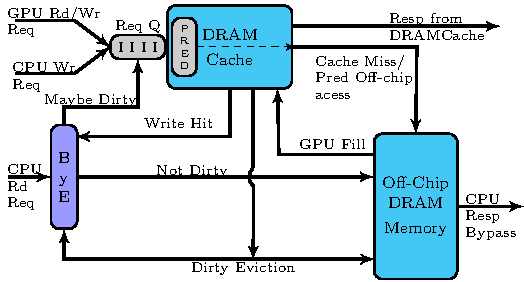
\includegraphics[scale=1.5]{figures/bloom}	
	\caption{Working of \cachename\ with \bypassname}
	\label{fig:bye}
\end{figure}

When the tag is matched in the DRAMCache, in the case of a hit, data from the DRAMCache is forwarded to the requester and the DRAM memory access is squashed or its response is ignored. In the case of a miss, data from the memory is forwarded and inserted into the cache. Normally, it is expected that the access to the DRAMCache completes earlier (due to its relatively lower access latency) than the DRAM response. However, when the GPU is running, the parallel request to off-chip DRAM memory often returns earlier and waits in the MSHRs. This is due to the increased queuing delay at the DRAMCache compared to the access latency at the DRAM. \cachename\ exploits this observation to bypass CPU read requests for both misses and clean lines.
\par For this, \cachename\ uses a Bypass Enabler (\bypassname). \bypassname\ uses a counting bloom filter \cite{bloom,counting-bloom} that tracks the dirty lines in the DRAMCache and provides a space efficient way to determine if a given request can be bypassed. The property of a bloom filter to answer "definitely not in set" allows us to bypass requests correctly i.e. without verifying tags in the set of the DRAMCache. 
On a write request when a cache line becomes dirty in the DRAMCache, the address is hashed into \bypassname\ and the corresponding counters are incremented. When a dirty line is evicted from the DRAMCache, \bypassname\ attempts to remove the entry from the Bloom filter by decrementing the corresponding locations \footnote{Counting bloom filters use saturating counters. If counter saturates, decrementing it can lead to false-negatives (dirty lines predicted as clean lines and wrongly bypassed). Hence saturated counters are never decremented.  While this may increase the false positives (clean lines being predicted as dirty), which only reduces the benefits obtained by \textit{ByE}, it does not affect functional correctness. In our implementation we observe that on an average just 2\% of 2-bit counters in the Bloom-filter saturate out of the 512K counters}.
\bypassname\ bypasses CPU requests only when the GPU cores are executing the kernel. For this, all CPU read requests lookup into \bypassname\ as shown in Figure \ref{fig:bye}. If the Bloom filter search returns a  negative result the address is guaranteed to be not dirty in the DRAMCache. Thus, the request can safely be bypassed to utilize the off-chip DRAM bandwidth. 
Further, when the bypassed CPU requests return from the off-chip DRAM access, these requests are directly forwarded to the requester and are not inserted into the cache. 
Firstly, this allows \bypassname\ to ensure that future write requests for the line do not hit in the DRAMCache as increase in dirty lines would lead to reduced bypass efficiency. 
% (we wanted this sentence cuz we dont want the reader to start thinking of reduced hit rates) Firstly, this allows \bypassname mechanism to continue bypassing future read requests for the line by ensuring that the write requests for  line do not hit in the cache causing reduced bypass efficiency
Secondly, this allows \bypassname\ to reduce some of the bloat caused by a Miss Fill \cite{bear} into the DRAMCache.
\par All write requests and GPU read requests proceed serially after looking into the cache. \bypassname\ does not bypass any write requests as it would otherwise require a back-invalidation of the cache line, if present in the DRAMCache, which would need a full DRAMCache access.
\par We find that a small 2-bit counting bloom filter implemented with two $H_3$ hash functions \cite{h3} and 512K entries per controller is sufficient 
to produce reasonable bypass efficiency with a tolerable mis-prediction rate. The total overhead for \bypassname\ is 256KB for a 64MB DRAMCache which is less than 0.4\% of the cache size.


\subsection{Heterogeneity aware Spatial Occupancy Control} \label{mechanism-chaining}
Objective: Allow GPU to better use DRAMCache Bandwidth
\par The schemes proposed in the previous two subsections, \prioname\ and \bypassname, attempt to improve the latency of CPU requests. The mechanism described in this section details \cachename's approach to improve the utilization of the DRAMCache for GPU requests, in order to exploit the higher bandwidth provided by it. We make the following observations and inferences: \textit{(i)} For the GPU to be able to better utilize the DRAMCache bandwidth, the hit rates for GPU workloads should be large enough that the GPU does not have to frequently use the relatively constricted off-chip DRAM buses. \textit{(ii)} As noted in Section \ref{motivation}, GPUs can trade access latencies for higher hit rates. Further, providing associativity for GPU requests improves the hit rate. \textit{(iii)} The working sets of CPU applications tend to be limited to few tens of MBs due to the limited amount of MLP that can be exploited by the CPUs. Thus, providing larger than certain share of cache leads to no further improvements in hit rates and IPC for CPU. Nevertheless, the CPU can still gain from some share of the DRAMCache due to reduced latency of access. \textit{(iv)} Given that GPU can exploit much higher MLP using several thousands of threads, the relatively small GPU L2 cache provides limited filtering of traffic and has significantly high miss rates while on the other hand CPUs have sufficiently sized L2 cache sizes to be able to retain blocks longer before re-requesting a block.
\par The above observations lead to the following conflicting requirements. It is important to ensure that the CPU requests have certain share (minimum occupancy) in the DRAMCache to ensure the benefits of lower latency while to effectively use the larger share of DRAMCache for GPU requests, it may be required to increase  associativity of the DRAMCache. However such an associativity should not unduly increase the hit latency for CPU requests. 
\par To accomplish the above goals, \cachename\ uses the \chaining\ scheme which introduces (pseudo) associativity mainly for GPU requests, while ensuring a certain minimum occupancy for CPU lines. The \chaining\ scheme uses a linear probing like technique inspired by the collision resolution mechanism of a hash map as shown in Figure \ref{fig:chaining-concept}.
To ensure minimum occupancy for CPU requests, \chaining\ maintains a low-threshold value (\textit{$l_{cpu}$}) and when the occupancy of CPU lines
\footnote{As mentioned earlier we classify a data as CPU data or GPU data based on whose request last accessed the data in the DRAMCache. An alternate equally feasible design point is to classify the data as CPU or GPU data based on which request brought the data into DRAMCache although the CPU and GPU may subsequently access it. In our setup only the CPU core executing the GPGPU application possibly shares data with the GPU and hence we do not expect to see significant difference in the results.} 
reaches this threshold, \chaining\ ensures GPU data does not replace data brought in by CPU. 

\begin{figure}
	\centering
	\def\svgwidth{0.45\linewidth}
	\input{figures/chainings.pdf_tex}
	\caption{Conceptual working of \chaining\ in \cachename}
	\label{fig:chaining-concept}
\end{figure}

In the other situations, \cachename\ modifies the replacement policy in the DRAMCache depending on the requesting core type. For a GPU request that is evicting another GPU line, \cachename\ looks for a line belonging to a CPU to replace within the same row in the next three consecutive locations,
i.e. if $B$ is the original cache block, then the blocks considered for insertions are $(B+1)\%N_s$,$(B+2)\%N_s$, and $(B+3)\%N_s$, where $N_s$ is number of blocks in a DRAMCache row (page). Hence, the inserted block always lies in the same row as the original cache block. Note that for every set, there could be at most 1 chained set, providing a pseudo-associativity of at most 1.  
We refer to this inserted location as the \textit{chained block} and the actual cache block the request mapped to as the \textit{original block}. The location of the \textit{chained block} is then represented as a 2-bit offset and is stored along with the metadata for the original set (see Figure \ref{fig:chain-access}(a)). When a cache block is evicted, if it was a \textit{chained block}, to unchain it (from the \textit{original block}), the offset stored in the reverse chain bits field in the metadata for the \textit{chained block} is used.  
The chain dirty bit field (Figure \ref{fig:chain-access}(a)) in the metadata indicates whether the chained location, if any, holds modified data. This is used to optimize the access path for CPU and reduce the adverse effect of a double set lookup for latency sensitive CPU requests as shown in Figure \ref{fig:chain-access}(b). \chaining\ relies on the hit/miss predictor to have started an early access to memory. This avoids the second set lookup for CPU if the parallel memory (PAM) access has returned and the chained block is clean. 


\begin{figure}[htb]
	\centering
	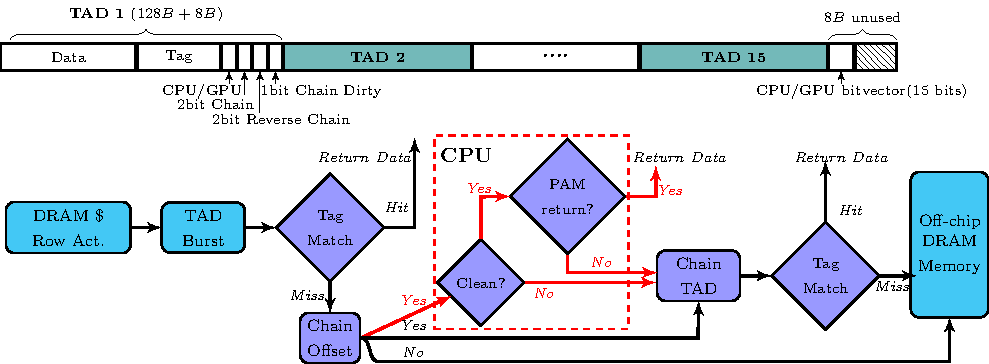
\includegraphics[scale=1]{figures/chaining}
	\caption{\cachename\ Row Organization and Access Path of a request}	
	\label{fig:chain-access}
\end{figure}

Additionally, each tag also stores 1 bit information about the owner of the block (CPU or GPU). This bit is used to make quick replacement decisions locally. The additional metadata required for \chaining\ is only 6 bits which can easily be accommodated in the existing 8 byte metadata. Lastly, the unused 8 byte (at the end of each row(page)) is used to store ownership information of each block in the row (15 bits). This information is used to make the \chaining\ replacement decision.


\par As explained earlier, when the \textit{$l_{cpu}$} threshold is reached, GPU lines are not allowed to evict CPU blocks and such GPU requests contending to evict a CPU line are forced to chain to another block belonging to a GPU and evicting that instead, thus maintaining the \textit{$l_{cpu}$} occupancy for CPU. In the very rare case that a GPU block is not found within the 3 consecutive locations the request is not inserted into the cache.

\begin{table}[htb]
	\centering
	\begin{tabular}{|c|c|c|c|c|}
\hline
\multirow{2}{*}{\begin{tabular}[c]{@{}l@{}}Threshold \\ Reached?\end{tabular}} & \multirow{2}{*}{\begin{tabular}[c]{@{}l@{}}Original\\ Set\end{tabular}} & \multirow{2}{*}{\begin{tabular}[c]{@{}l@{}}Not \\ Chained\end{tabular}} & \multicolumn{2}{c|}{Chained Set}                                                                                         \\ \cline{4-5} 
                                                                               &                                                                         &                                                                         & CPU                                                        & GPU                                                        \\ \hline
\multirow{2}{*}{No}                                                             & CPU                                                                     & \begin{tabular}[c]{@{}l@{}}replace\\ original\end{tabular}              & \begin{tabular}[c]{@{}l@{}}replace\\ chained\end{tabular}  & \begin{tabular}[c]{@{}l@{}}replace\\ original\end{tabular} \\ \cline{2-5} 
                                                                               & GPU                                                                     & \begin{tabular}[c]{@{}l@{}}Chain to\\ nearest \\ CPU set\end{tabular}   & \begin{tabular}[c]{@{}l@{}}replace\\ chained\end{tabular}  & \begin{tabular}[c]{@{}l@{}}replace\\ original\end{tabular} \\ \hline
\multirow{2}{*}{Yes}                                                             & CPU                                                                     & \begin{tabular}[c]{@{}l@{}}Chain to\\ nearest\\ GPU Set\end{tabular}    & \begin{tabular}[c]{@{}l@{}}do not\\ insert\end{tabular}    & \begin{tabular}[c]{@{}l@{}}replace\\ chained\end{tabular}  \\ \cline{2-5} 
                                                                               & GPU                                                                     & \begin{tabular}[c]{@{}l@{}}replace\\ original\end{tabular}              & \begin{tabular}[c]{@{}l@{}}replace\\ original\end{tabular} & \begin{tabular}[c]{@{}l@{}}replace\\ original\end{tabular} \\ \hline
\end{tabular}
	\caption{\chaining\ mechanism GPU Fill request insertion policy. }
	\label{chaining-replacement}
\end{table}

\par We now summarize the insertion policy used by \chaining\ mechanism in \cachename. 
\par For all CPU fill (insertion) requests, the data is always inserted in the original block, and the victim block is evicted - removing chaining, if any, using the reverse chain bit. 
\par The memory controller maintains a running GPU occupancy counter for each row in the DRAMCache. This information is accomodated in the unused bits at the end of the row in the DRAMCache and can be cached in SRAM structures for fast lookups. Using this current occupancy counter the controller decides the fill policy for the GPU fill request. The threshold reached is determined by comparing the current GPU occupany with the set \textit{$l_{cpu}$} threshold value as : $O_{gpu}\le(1-l_{cpu})$ where $O_{gpu}$ is the current GPU occupancy in DRAMCache row. For a GPU fill request, if the low threshold mark for CPU occupancy is not reached, then the \chaining\ scheme replaces a CPU location, either from the original location or from the chained location, as indicated in row 1 of Table \ref{chaining-replacement}. For a GPU fill request, if the original location belongs to GPU and does not have a chained location, then block is inserted in one of the nearest CPU block [$(B+1)\%N_s$ or $(B+2)\%N_s$ or $(B+3)\%N_s$]. If such a nearest CPU block is not found, the request is inserted into original block itself. If the original location is chained, then the scheme replaces the chained location, if that belongs to CPU or the original location itself, as indicated in row 2 of Table \ref{chaining-replacement}. When the CPU occupancy has hit low threshold, then a GPU fill request replaces the original location if it belongs to GPU (row 4 in Table \ref{chaining-replacement}). If the original location belongs to CPU and does not have a chained block, then the GPU request is chained to the next nearest GPU location. If the original location is chained, but the chained location belongs to GPU, then the fill request replaces that. Otherwise, the fill request is not inserted in the DRAMCache (see row 3 in Table \ref{chaining-replacement}). Thus the \chaining\ scheme ensures, as far as possible, the CPU requests can find the data in the original location, while the GPU requests attempt to exploit pseudo associativity for increased cache occupancy. In all cases (for both GPU and CPU requests) the access is satisfied with at most 2 tag matches, either in original location or in the chained location (identified by the chain bits). 

\par In essence, \cachename\ uses this \chaining\ mechanism to force occupancy control in the DRAMCache. \chaining\ is able to 
(i) ensure a minimum occupancy for the CPU lines while effectively allowing the GPU to occupy the rest of the DRAMCache by providing pseudo-associativity;
(ii) remain as a direct mapped cache for majority of the CPU requests; and
(iii) avoid forcing eviction of hot GPU lines while also avoiding storing of dead lines in the cache.
Lastly, this scheme is dynamic and allows to adaptively set CPU occupancy threshold \textit{$l_{cpu}$} based on the workloads requirements. This occupancy control mechanism does not incur any additional storage and uses the unused space in the DRAMCache rows. Once the GPU finishes kernel execution \cachename\ returns to a direct mapped cache as the CPU lines inserted into the DRAMCache occupy \textit{chained blocks} thereby unlinking chains. 

\vspace{-1em}
\section{Summary}
In this chapter we presented the \cachename\ organization and mechanisms. We firstly showed the conscientious design designs made and substantiated them with experiments of DRAMCache for IHS architecture. We then details the principle and workings of \prioname, \bypassname\ and \chaining\ mechanisms in the \cachename.

